%!TeX root = thesis-main.tex
\begin{figure}[!ht]
  \begin{comment}
  \begin{subfigure}[b]{0.32\textwidth}
    \centering
    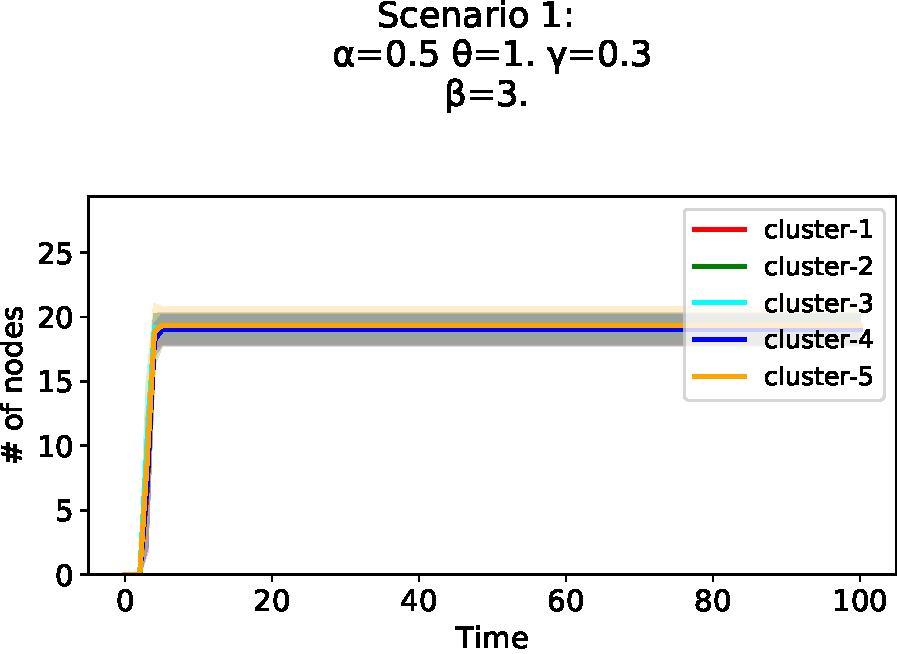
\includegraphics[width=\textwidth]{papers/swarm-intelligence2021/img/simulations/standard-count_0_034567_α-0.5_θ-1._γ-0.3_β-3._ω-0._ζ-0..pdf}
  \end{subfigure}
  \hfill
  \begin{subfigure}[b]{0.32\textwidth}
    \centering
    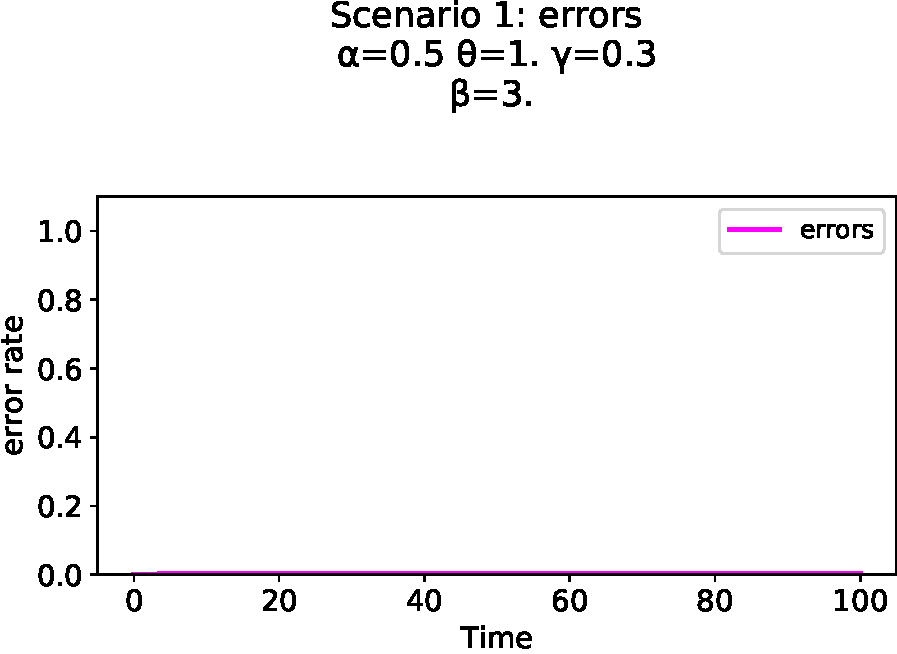
\includegraphics[width=\textwidth]{papers/swarm-intelligence2021/img/simulations/standard-errors_0_08_α-0.5_θ-1._γ-0.3_β-3._ω-0._ζ-0..pdf}
  \end{subfigure}
  \hfill
  \begin{subfigure}[b]{0.32\textwidth}
    \centering
    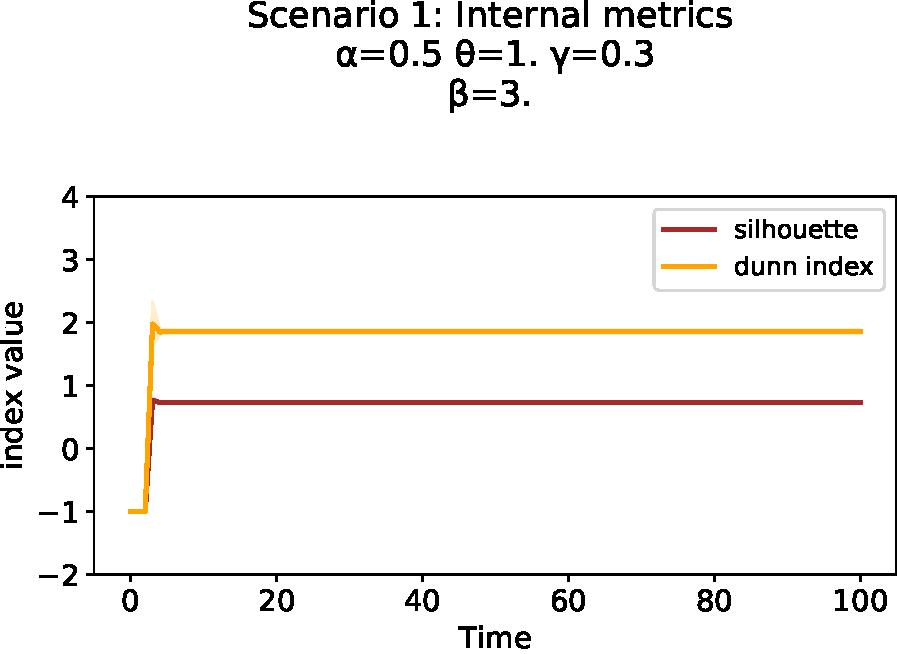
\includegraphics[width=\textwidth]{papers/swarm-intelligence2021/img/simulations/standard-metrics_0_0910_α-0.5_θ-1._γ-0.3_β-3._ω-0._ζ-0..pdf}
  \end{subfigure}
  \\
\end{comment}
  \begin{subfigure}[b]{0.32\textwidth}
    \centering
    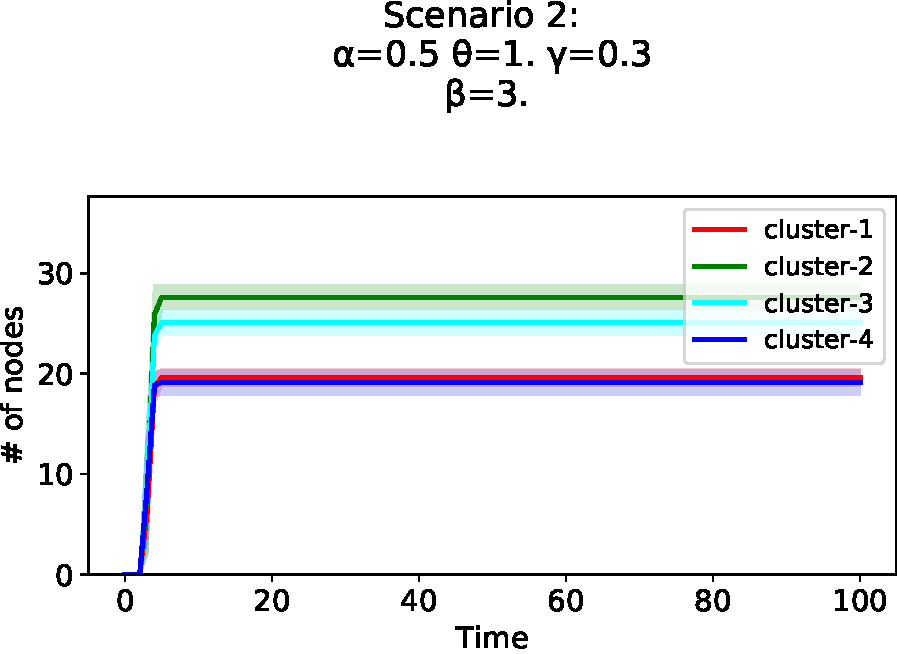
\includegraphics[width=\textwidth]{papers/swarm-intelligence2021/img/simulations/stretched-count_0_03456_α-0.5_θ-1._γ-0.3_β-3._ω-0._ζ-0..pdf}
  \end{subfigure}
  \hfill
  \begin{subfigure}[b]{0.32\textwidth}
    \centering
    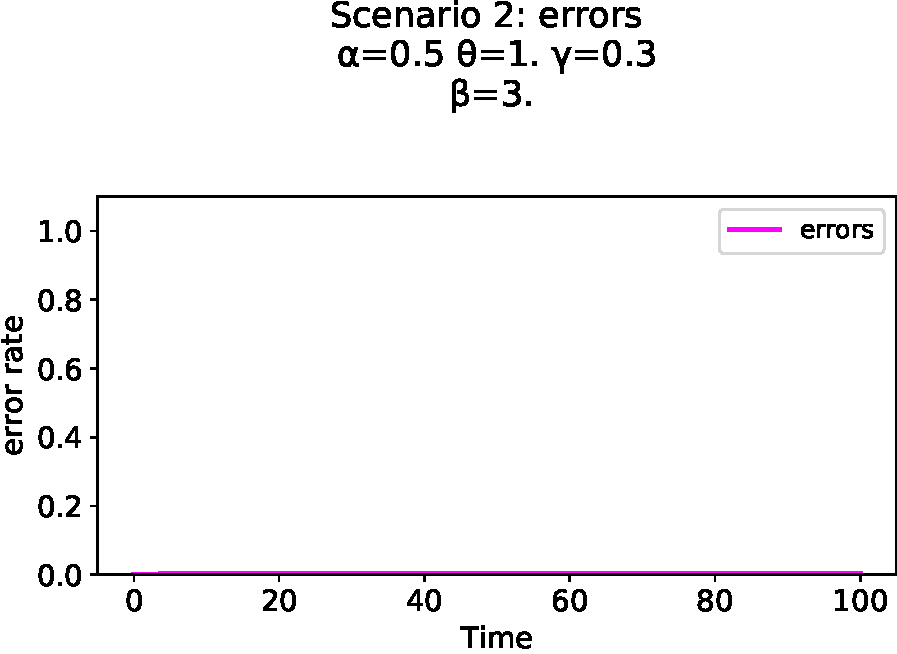
\includegraphics[width=\textwidth]{papers/swarm-intelligence2021/img/simulations/stretched-errors_0_08_α-0.5_θ-1._γ-0.3_β-3._ω-0._ζ-0..pdf}
  \end{subfigure}
  \hfill
  \begin{subfigure}[b]{0.32\textwidth}
    \centering
    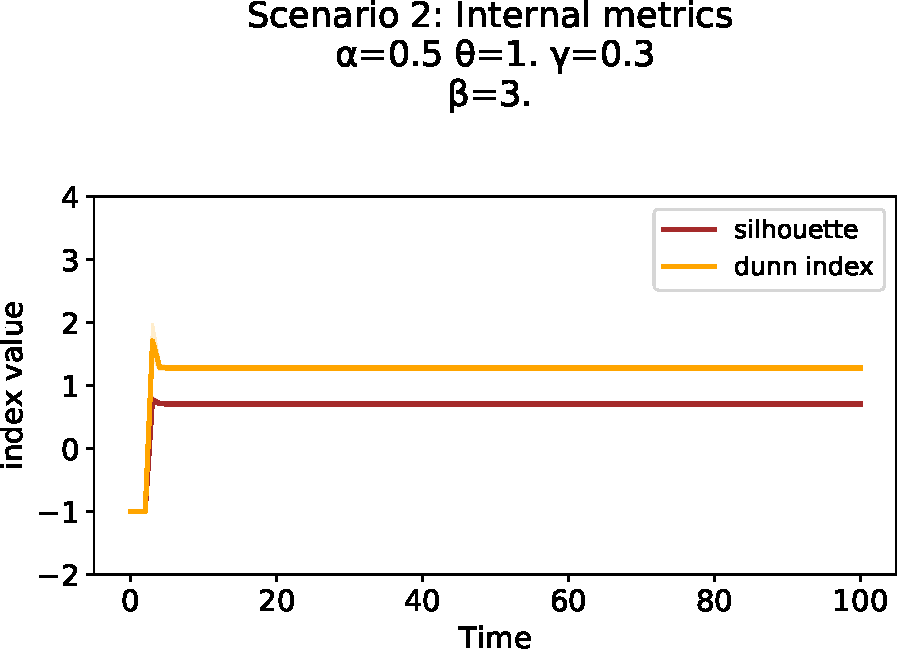
\includegraphics[width=\textwidth]{papers/swarm-intelligence2021/img/simulations/stretched-metrics_0_0910_α-0.5_θ-1._γ-0.3_β-3._ω-0._ζ-0..pdf}
  \end{subfigure}
  \\
  \begin{subfigure}[b]{0.32\textwidth}
    \centering
    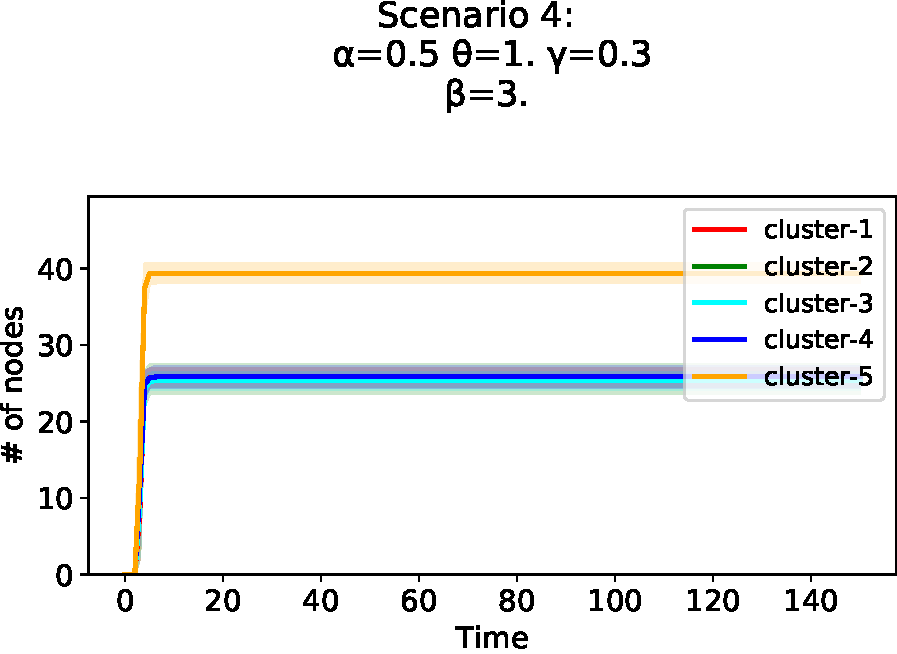
\includegraphics[width=\textwidth]{papers/swarm-intelligence2021/img/simulations/overlay-count_0_034567_α-0.5_θ-1._γ-0.3_β-3._ω-0._ζ-0..pdf}
  \end{subfigure}
  \hfill
  \begin{subfigure}[b]{0.32\textwidth}
    \centering
    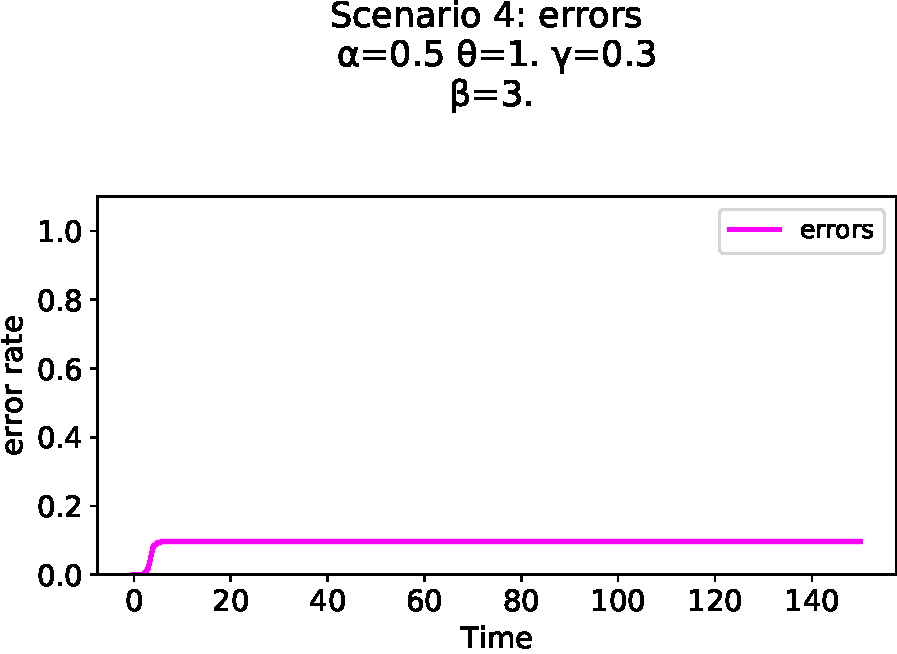
\includegraphics[width=\textwidth]{papers/swarm-intelligence2021/img/simulations/overlay-errors_0_08_α-0.5_θ-1._γ-0.3_β-3._ω-0._ζ-0..pdf}
  \end{subfigure}
  \hfill
  \begin{subfigure}[b]{0.32\textwidth}
    \centering
    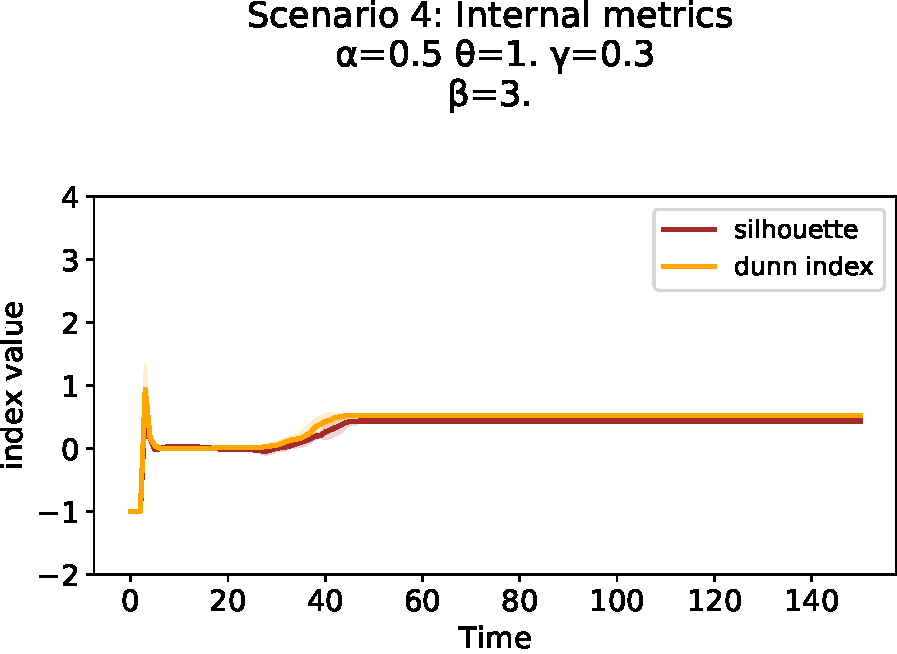
\includegraphics[width=\textwidth]{papers/swarm-intelligence2021/img/simulations/overlay-metrics_0_0910_α-0.5_θ-1._γ-0.3_β-3._ω-0._ζ-0..pdf}
  \end{subfigure}
  \\
  \begin{subfigure}[b]{0.32\textwidth}
    \centering
    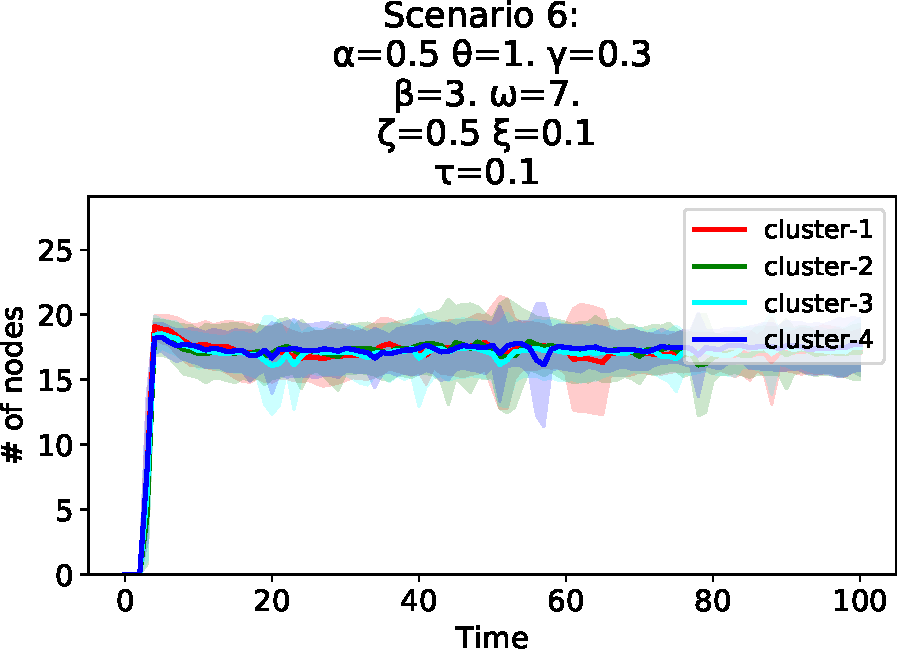
\includegraphics[width=\textwidth]{papers/swarm-intelligence2021/img/simulations/movement-count_0_03456_α-0.5_θ-1._γ-0.3_β-3._ω-7._ζ-0.5.pdf}
  \end{subfigure}
  \hfill
  \begin{subfigure}[b]{0.32\textwidth}
    \centering
    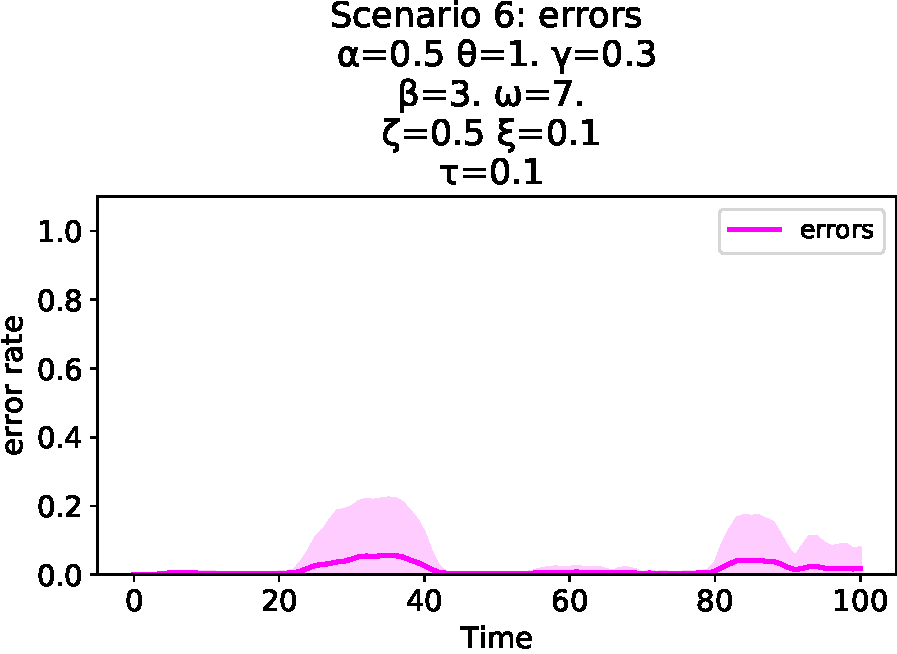
\includegraphics[width=\textwidth]{papers/swarm-intelligence2021/img/simulations/movement-errors_0_08_α-0.5_θ-1._γ-0.3_β-3._ω-7._ζ-0.5.pdf}
  \end{subfigure}
  \hfill
  \begin{subfigure}[b]{0.32\textwidth}
    \centering
    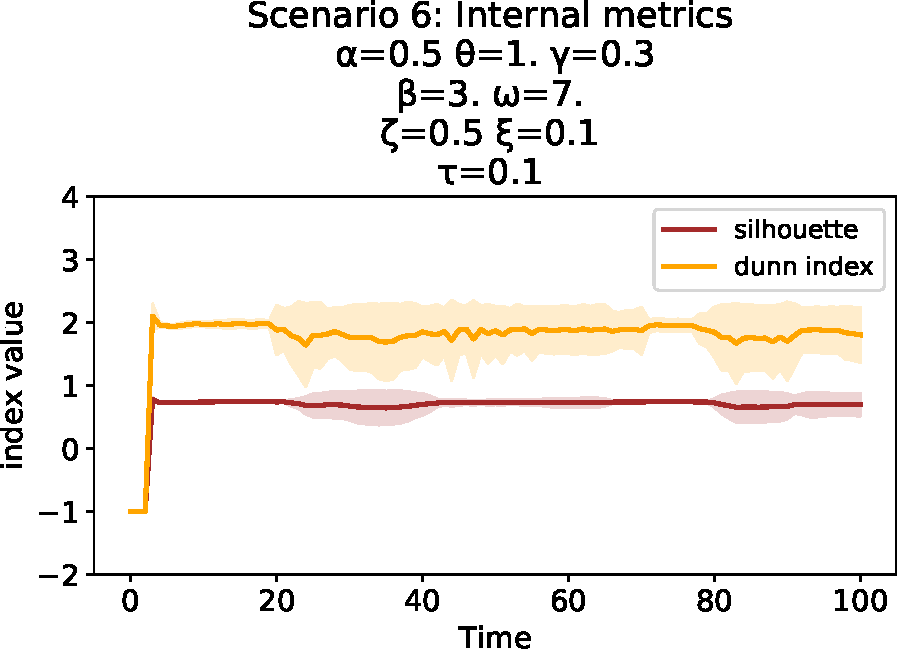
\includegraphics[width=\textwidth]{papers/swarm-intelligence2021/img/simulations/movement-metrics_0_0910_α-0.5_θ-1._γ-0.3_β-3._ω-7._ζ-0.5.pdf}
  \end{subfigure}
  \\
  \begin{subfigure}[b]{0.32\textwidth}
    \centering
    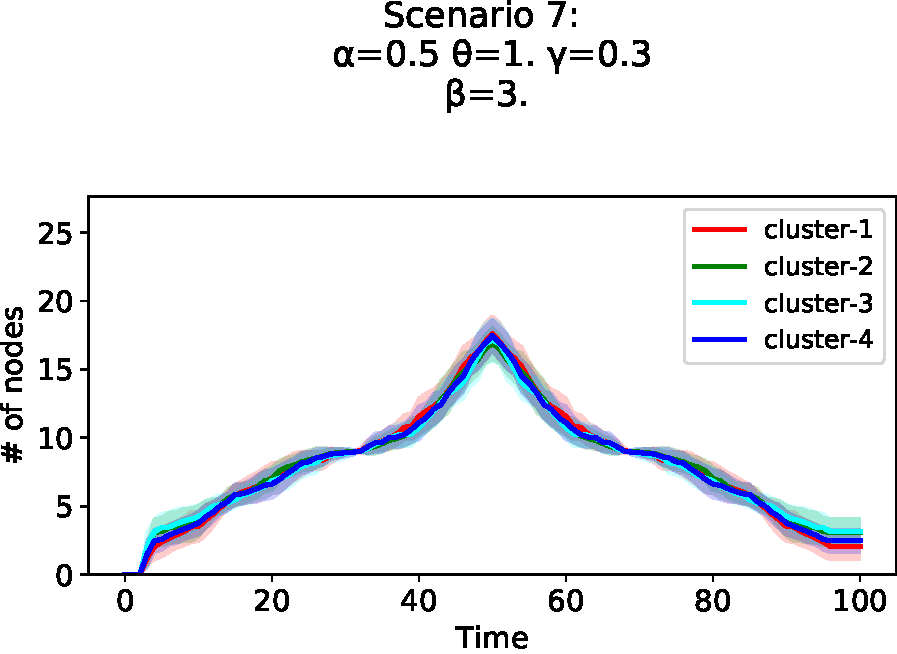
\includegraphics[width=\textwidth]{papers/swarm-intelligence2021/img/simulations/standard-updatable-count_0_03456_α-0.5_θ-1._γ-0.3_β-3._ω-0._ζ-0..pdf}
  \end{subfigure}
  \hfill
  \begin{subfigure}[b]{0.32\textwidth}
    \centering
    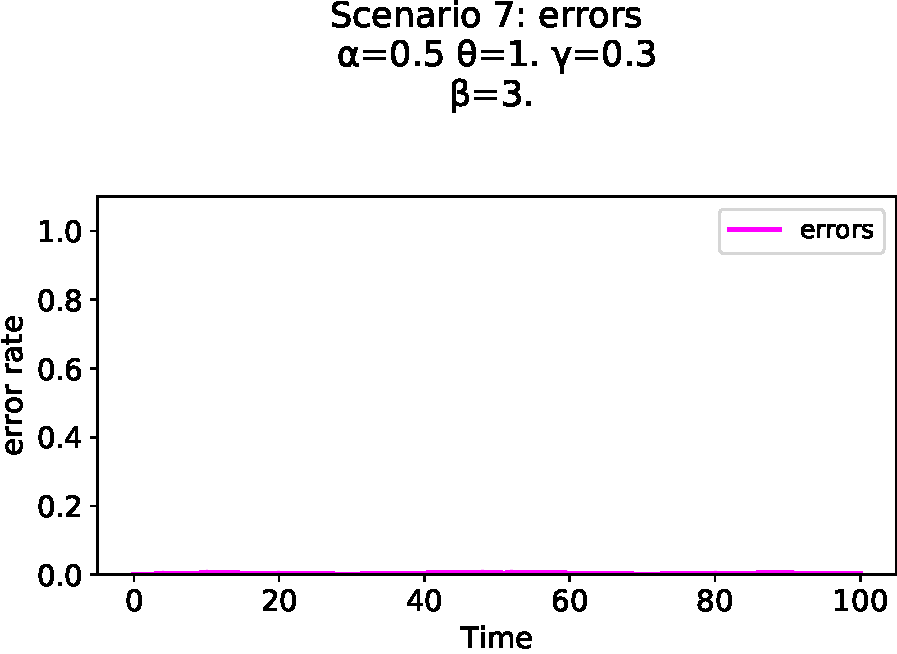
\includegraphics[width=\textwidth]{papers/swarm-intelligence2021/img/simulations/standard-updatable-errors_0_08_α-0.5_θ-1._γ-0.3_β-3._ω-0._ζ-0..pdf}
  \end{subfigure}
  \hfill
  \begin{subfigure}[b]{0.32\textwidth}
    \centering
    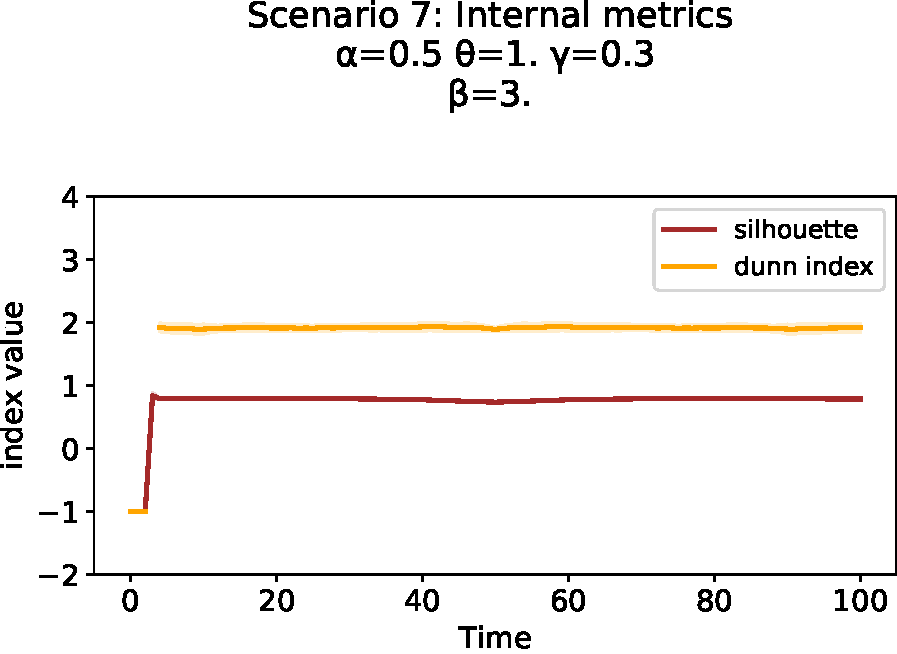
\includegraphics[width=\textwidth]{papers/swarm-intelligence2021/img/simulations/standard-updatable-metrics_0_0910_α-0.5_θ-1._γ-0.3_β-3._ω-0._ζ-0..pdf}
  \end{subfigure}
  \\
  \begin{subfigure}[b]{0.32\textwidth}
    \centering
    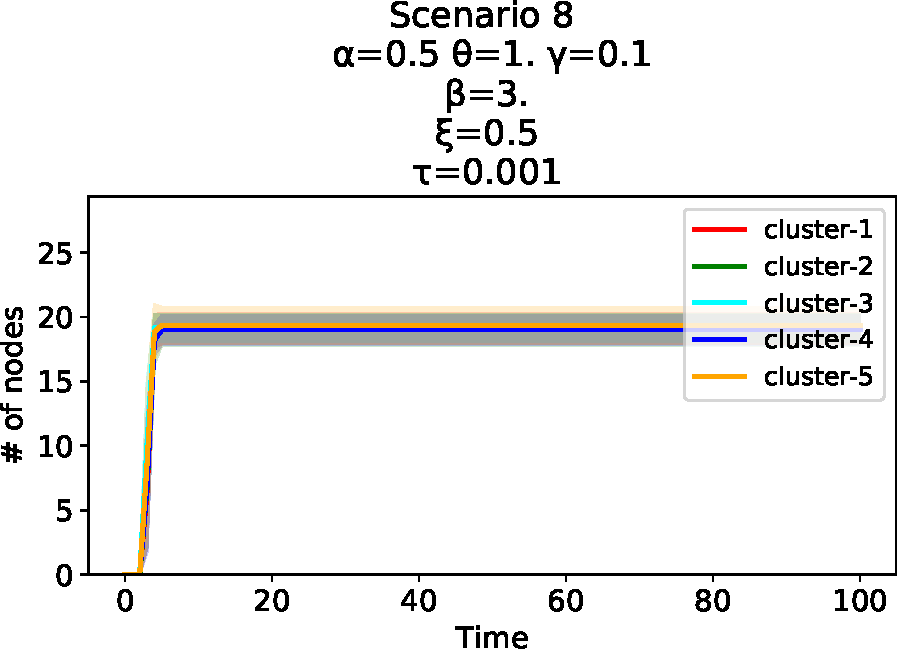
\includegraphics[width=\textwidth]{papers/swarm-intelligence2021/img/simulations/failScenario_0_034567_α-0.5_θ-1._γ-0.1_β-3._ω-0._ζ-0._ξ-0.5_τ-0.001}
  \end{subfigure}
  \hfill
  \begin{subfigure}[b]{0.32\textwidth}
    \centering
    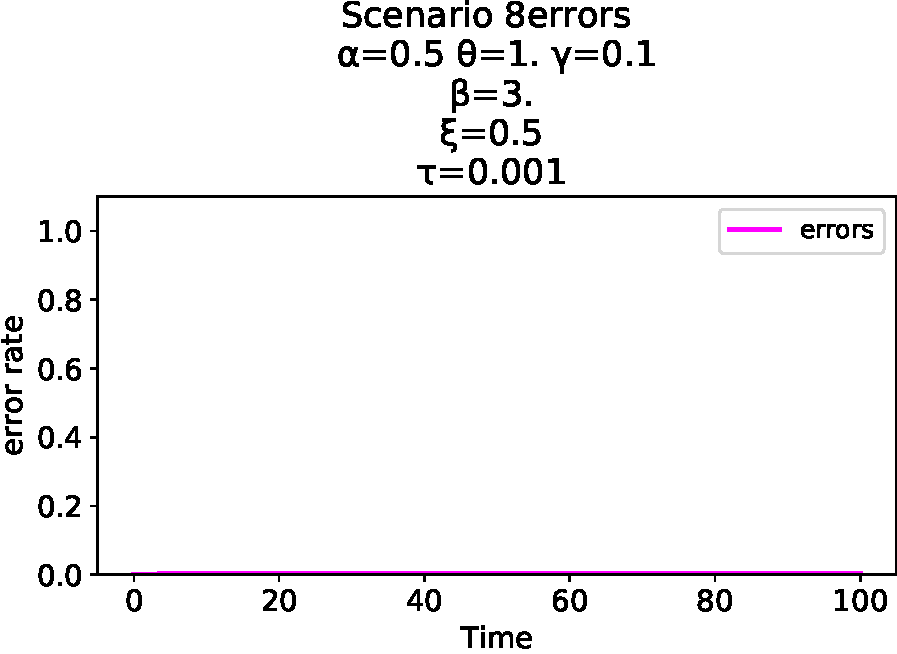
\includegraphics[width=\textwidth]{papers/swarm-intelligence2021/img/simulations/failScenario_0_08_α-0.5_θ-1._γ-0.1_β-3._ω-0._ζ-0._ξ-0.5_τ-0.001}
  \end{subfigure}
  \hfill
  \begin{subfigure}[b]{0.32\textwidth}
    \centering
    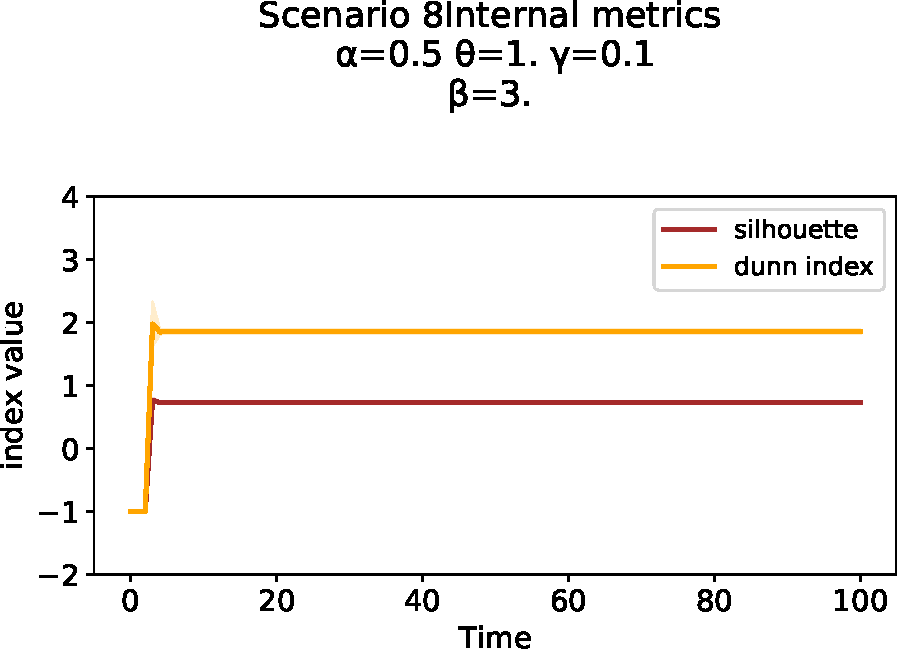
\includegraphics[width=\textwidth]{papers/swarm-intelligence2021/img/simulations/failScenario_0_0910_α-0.5_θ-1._γ-0.1_β-3._ω-0._ζ-0._ξ-0.5_τ-0.001}
  \end{subfigure}
  \caption[In-depth analysis of good clustering results.]{In-depth analysis of good simulation results. 
  In general, the algorithm produces good results. 
  \rev{In the case of movement and failures, the error can reach up to 10 per cent.}}
  
  \label{fig:good-simulation-results}
\end{figure}